%%%%%%%%%%%%%%%%%%%
%% A R B I T E R %%
%%%%%%%%%%%%%%%%%%%

\subsection{Arbiter}
\label{subsec:arbiter}

The Arbiter controls access to the memory interface shared by read and write requests. It implements a round-robin arbitration policy.

The arbiter maintains a priority state indicating which request type has priority when read (channel $a$) and write (channel $b$) requests are asserted simultaneously. When only one request is active, that request is granted regardless of the current priority. When both requests are active, the request with the current priority is granted. After a request is granted, the priority is updated to favor the other request type.

\begin{figure}[H]
	\centering
	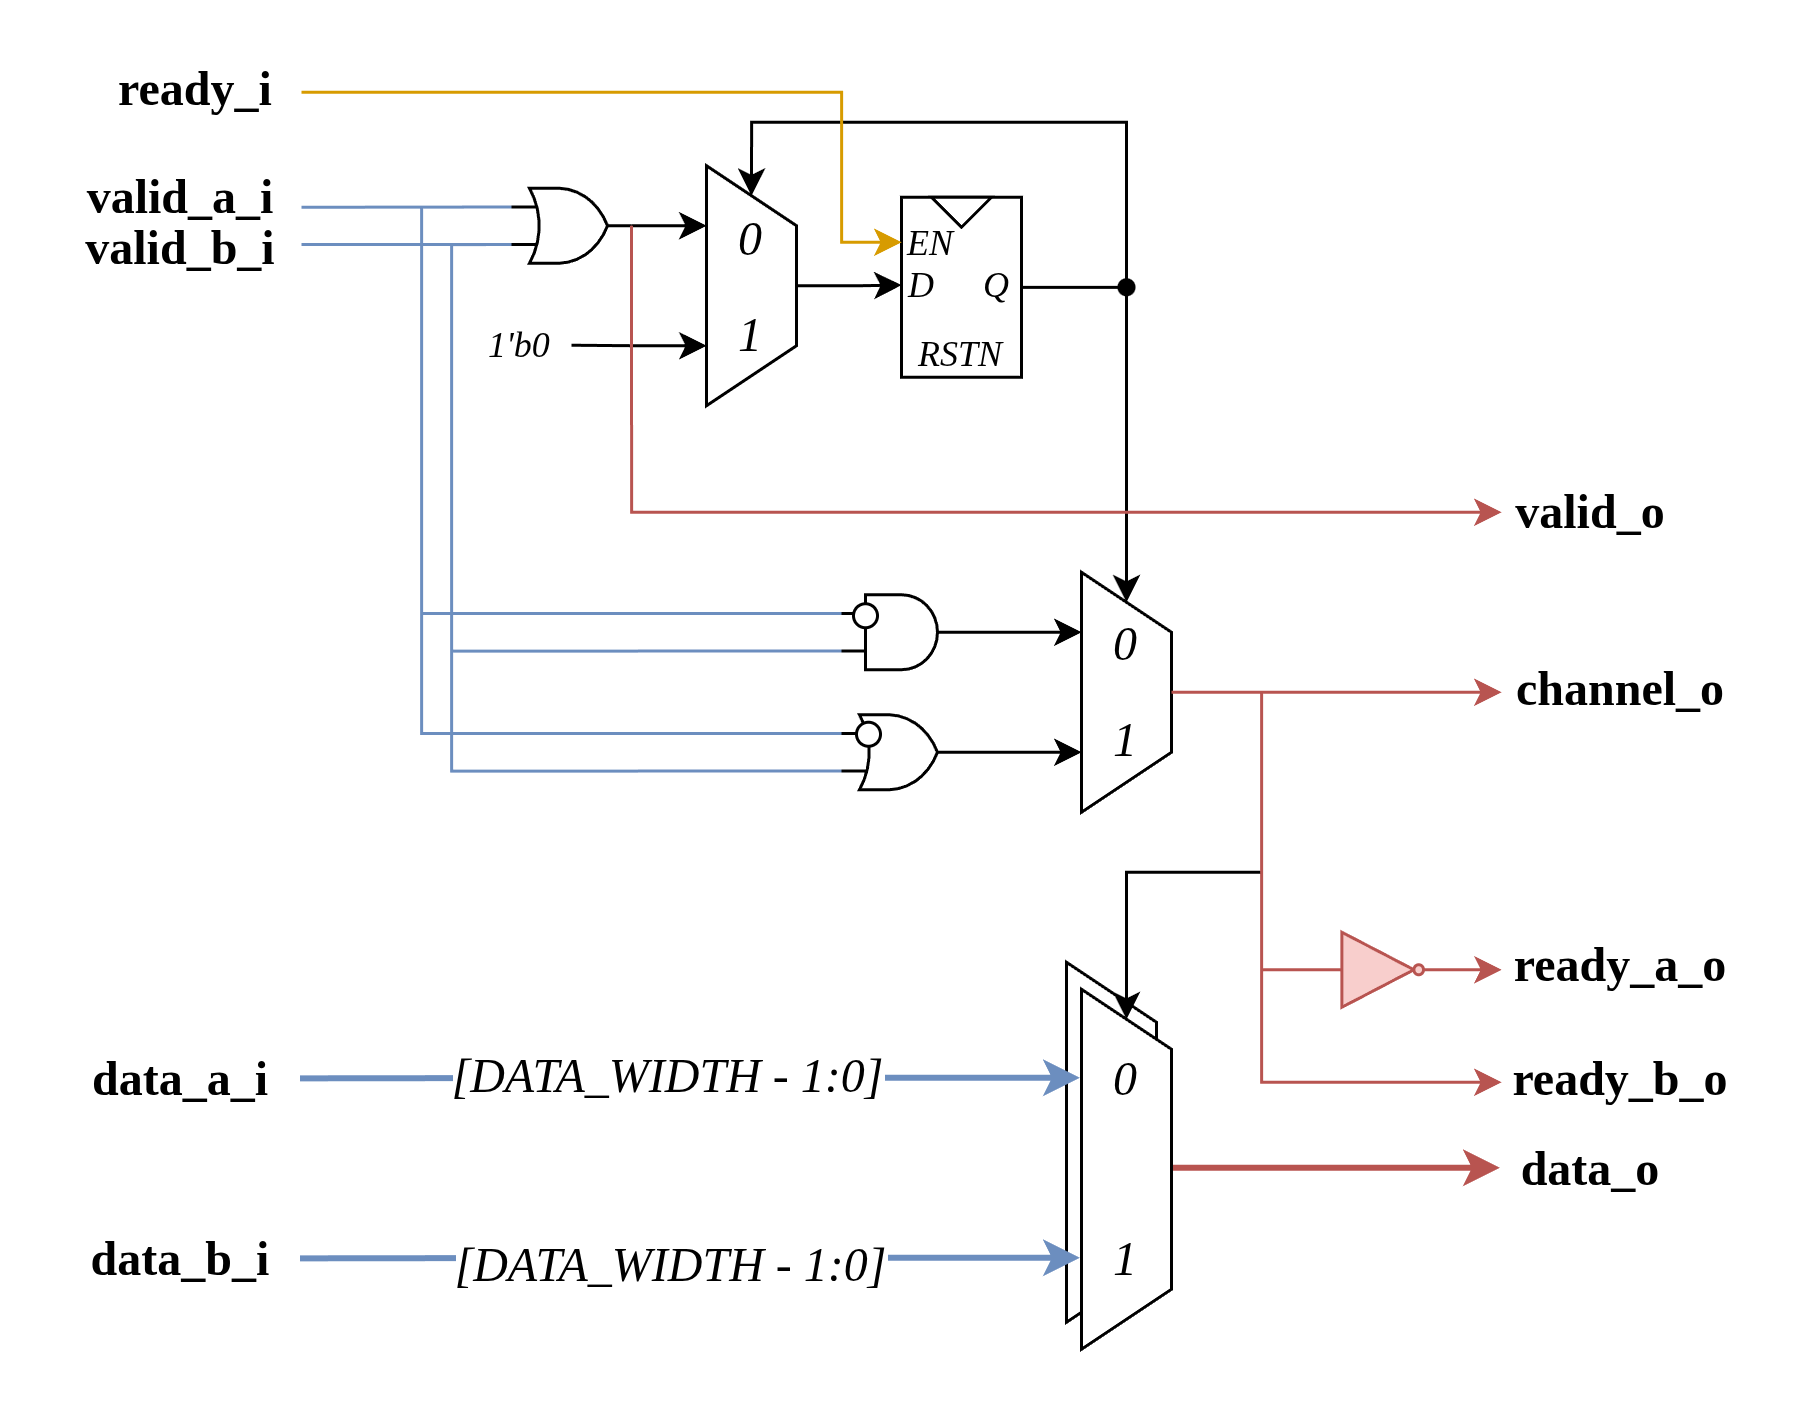
\includegraphics[width=7cm]{Arbiter.png}
	\caption{Round-Robin arbiter scheme}
\end{figure}

\begin{table}[H]
	\centering
	\small
	\begin{tabularx}{\textwidth}{l c c X}
		\toprule
		\textbf{Parameter} & \textbf{Valid Range} & \textbf{Default} & \textbf{Description} \\
		\midrule
		
		\verb|DATA_WIDTH| &
		Positive integer &
		\verb|32| &
		Width of the transaction data path. \\
		
		\bottomrule
	\end{tabularx}
	\caption{Round-Robin Arbiter parameters}
	\label{tab:round_robin_arbiter_parameters}
\end{table}

\begin{table}[H]
	\centering
	\label{tab:round_robin_arbiter_ports}
	\small
	\begin{tabularx}{\textwidth}{l c c X}
		\toprule
		\textbf{Ports} & \textbf{Direction} & \textbf{Width} & \textbf{Description} \\
		\midrule
		
		\verb|ready_i| &
		Input &
		\verb|1| &
		Indicates that the downstream logic is ready to accept the selected transaction. \\
		
		\verb|valid_a_i| &
		Input &
		\verb|1| &
		Indicates that a valid transaction is available on channel A. \\
		
		\verb|data_a_i| &
		Input &
		\verb|DATA_WIDTH| &
		Transaction data provided on channel A. \\
		
		\verb|valid_b_i| &
		Input &
		\verb|1| &
		Indicates that a valid transaction is available on channel B. \\
		
		\verb|data_b_i| &
		Input &
		\verb|DATA_WIDTH| &
		Transaction data provided on channel B. \\
		
		\verb|ready_o| &
		Output &
		\verb|1| &
		Indicates that arbiter is ready. \\
		
		\verb|valid_o| &
		Output &
		\verb|1| &
		Indicates that a valid transaction is available at the output. \\
		
		\verb|data_o| &
		Output &
		\verb|DATA_WIDTH| &
		Transaction data selected by the arbiter. \\
		
		\bottomrule
	\end{tabularx}
	\caption{Round-Robin Arbiter ports}
\end{table}